\begin{figure}
    \centering
    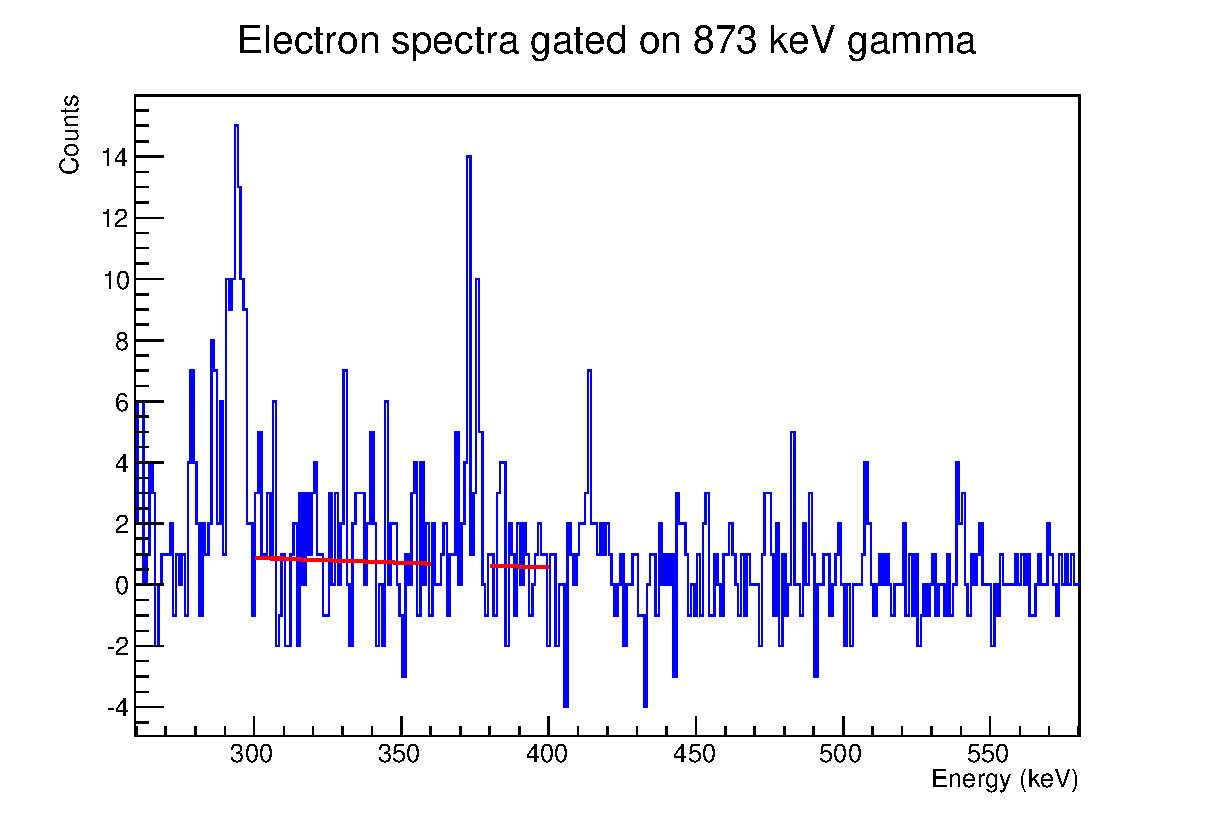
\includegraphics[scale=0.6]{Analysis_Figs/Piecewise_example.eps}
    \caption[An example of the global background fit used for peaks that could not be fit using the skewed gaussian function.]{An example of the global background fit used for peaks that could not be fit using the skewed gaussian function. The areas on either side of the peak are selected by the user. Once the background fit is done, the central area between the two sections is treated as the peak and the background is subtracted off to give a peak area. The red line shows the fit for the background area, and the two sections used for the background fit. See \ref{chap:macro} for the global-fit function used.}
    \label{fig:piecewise}
\end{figure}